\documentclass[xcolor=dvipsnames,table]{beamer}

\usepackage{latexsym}
\usepackage[utf8]{inputenc}
\usepackage[brazil]{babel}
\usepackage{amssymb}
\usepackage{amsmath}
\usepackage{stmaryrd}
\usepackage{fancybox}
\usepackage{datetime}
\usepackage[T1]{fontenc}
\usepackage{graphicx}
\usepackage{graphics}
\usepackage{url}
\usepackage{algorithmic}
\usepackage{algorithm}
\usepackage{acronym}
\usepackage{array}
\usepackage[normalem]{ulem}

\newtheorem{definicao}{Definio}
\newcommand{\tab}{\hspace*{2em}}

\mode<presentation>
{
  \definecolor{colortexto}{RGB}{0,0,0}
 
  \setbeamertemplate{background canvas}[vertical shading][ bottom=white!10,top=white!10]
  \setbeamercolor{normal text}{fg=colortexto} 

  \usetheme{Warsaw}
}

\title{Classe NP-Completa} 

\author{
  Esdras Lins Bispo Jr. \\ \url{bispojr@ufg.br}
  } 
 \institute{
  Teoria da Computação \\Bacharelado em Ciência da Computação}
\date{\textbf{01 de agosto de 2016} }

\logo{
\includegraphics[width=1cm]{images/ufgJataiLogo.png}}

\begin{document}

	\begin{frame}
		\titlepage
	\end{frame}

	\AtBeginSection{
		\begin{frame}{Sumário}%[allowframebreaks]{Sumário}
    		\tableofcontents[currentsection]
    		%\tableofcontents[currentsection, hideothersubsections]
		\end{frame}
	}

	\begin{frame}{Plano de Aula}
		\tableofcontents
		%\tableofcontents[hideallsubsections]
	\end{frame}
    
    \section{Pensamento}
	\begin{frame}{Pensamento}
  		\begin{center}
    		
\includegraphics[width=7cm]{images/pensamento.png}
  		\end{center}
	\end{frame}
	
	\begin{frame}{Pensamento}
		\begin{columns}
			\column{.4\textwidth}  		
		  		\begin{center}
		    		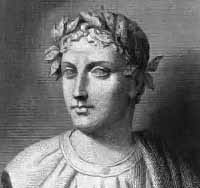
\includegraphics[height=.5\textheight]{images/horacio.jpg}
		  		\end{center}
			\column{.6\textwidth}  		
				\begin{block}{Frase}
					\begin{center}
						{\large A força bruta, quando não é governada pela razão, desmorona sob o seu próprio peso.}
					\end{center}
				\end{block}		  		
		  		\begin{block}{Quem?}
		  			\begin{center}
						{\bf Quinto Horácio (65 a.C. - 8 a.C.)} \\ Filósofo e poeta romano.
					\end{center}
				\end{block}
		\end{columns}
	\end{frame}
	
%------------------------------------------

\section{Revisão}
	
	\subsection{Classe NP}				
	
	\begin{frame}{A Classe NP}
		\begin{block}{Problema do {\bf caminho hamiltoniano} em um grafo}
			$CAMHAM = \{ \langle G, s, t \rangle \mbox{ | } G$ é um grafo direcionado com um caminho hamiltoniano de $s$ para $t \}$.
		\end{block}
		\begin{center}
			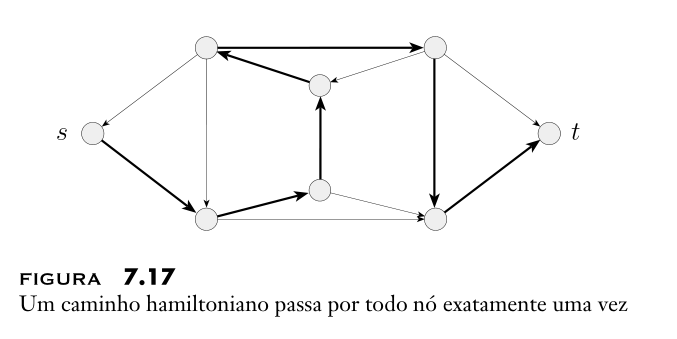
\includegraphics[width=9cm]{images/camHam.png}
		\end{center}
	\end{frame}	
	
	\begin{frame}[shrink]{Classe NP}
		\begin{block}{Característica importante}
			O problema $CAMHAM$ tem {\bf verificabilidade polinomial}
		\end{block} 
		\begin{block}{Outro problema polinomialmente verificável...}
			$COMPOSTOS = \{ x$ | $x = pq$, para inteiros $p,q > 1 \}$
		\end{block} 
		\begin{exampleblock}{Exemplo}
			$33 \in COMPOSTOS$ $\therefore$ 
			\begin{itemize}
				\item $3 \times 11 = 33$
				\item $3, 11 \in \mathbb{Z}$
			\end{itemize}
		\end{exampleblock} 
		\begin{alertblock}{Porém...}
			Existem problemas que não podem ser verificados em tempo polinomial. Exemplo: $\overline{CAMHAM}$.
		\end{alertblock}
	\end{frame}
	
	\begin{frame}{Classe NP}
		\begin{block}{Definição 7.18}
			Um {\bf verificador} para uma linguagem $A$ é um algoritmo $V$, em que
			\begin{center}
				$A = \{ \omega$ | $V$ aceita $\langle \omega, c \rangle$ para alguma cadeia $c \}$.
			\end{center}
		\end{block} 
		\begin{block}{Detalhes}
			Medimos o tempo de um verificador somente em termos do comprimento de $\omega$, portanto um {\bf verificador de tempo polinomial} roda em tempo polinomial no comprimento de $\omega$. 
		\end{block} 
		\begin{block}{Nomenclaturas...}
			Uma linguagem $A$ é {\bf polinomialmente verificável} se ela tem um verificador de tempo polinomial.
		\end{block}
	\end{frame}		
	
	\begin{frame}{Classe NP}
		\begin{block}{Certificado (Prova)}
			\begin{itemize}
				\item A informação adicional, representada por $c$, utilizada por um verificador é chamada de {\bf certificado} (ou prova) da pertinência a uma dada linguagem. 
				\item Para verificadores polinomiais, o certificado tem comprimento polinomial (no comprimento de $\omega$).
			\end{itemize}
		\end{block} 
		\begin{block}{Exemplo}
			\begin{itemize}
				\item Um certificado para uma cadeia $\langle G, s, t \rangle \in CAMHAM$ é um caminho hamiltoniano de $s$ a $t$. 
				\item Um certificado para um número composto $x \in COMPOSTOS $ é um dos seus divisores.
			\end{itemize}
		\end{block}
	\end{frame}
	
	\begin{frame}[shrink]{Classe NP}
		\begin{block}{Definição 7.19}
			{\bf NP} é a classe das linguagens que têm verificadores de tempo polinomial.
		\end{block}
		\begin{block}{Teorema 7.20}
			Uma linguagem está em {\bf NP} sse ela é decidida por alguma máquina de Turing não-determinística de tempo polinomial.
		\end{block} 
		\begin{block}{Definição 7.21}
			{\bf NTIME(t(n))} = $\{L$ | $L$ é uma linguagem decidida por uma MT não-determinística de tempo $O(t(n)) \}$.
		\end{block}
		\begin{exampleblock}{Corolário}
			{\bf NP} $ \cong \bigcup_k$ {\bf NTIME($n^k$)}
		\end{exampleblock}
	\end{frame}
	
	\subsection{CLIQUE}
	\begin{frame}{A Classe NP}
		\begin{block}{Problema do clique em um grafo}
			$CLIQUE = \{ \langle G, k \rangle \mbox{ | } G$ é um grafo não-direcionado com um $k$-clique $\}$.
		\end{block}
		\begin{center}
			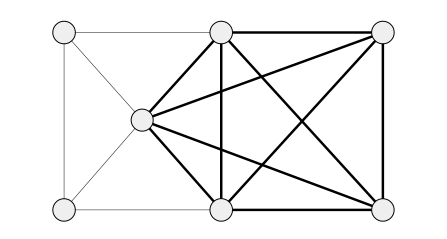
\includegraphics[width=8cm]{images/clique.png}
		\end{center}
	\end{frame}	
	
	\begin{frame}{A Classe NP}
		\begin{block}{Teorema 7.24}
			CLIQUE $\in$ {\bf NP}
		\end{block} 
		\begin{block}{Prova (usando o clique $c$ como certificado para $V$)}
			$V$ = ``Sobre a cadeia de entrada $\langle \langle G, k \rangle, c \rangle$:
			\begin{enumerate}
				\item Teste se $c$ é um conjunto de $k$ nós em $G$;
				\item Teste se $G$ contém todas as arestas conectando nós em $c$;
				\item Se ambos os testes retornam positivo, {\it aceite}. Caso contrário, {\it rejeite}.
			\end{enumerate}
		\end{block}
	\end{frame}
	
	\begin{frame}{A Classe NP}
		\begin{block}{Teorema 7.24}
			CLIQUE $\in$ {\bf NP}
		\end{block} 
		\begin{block}{Prova (construindo a MTN $M$)}
			$M$ = ``Sobre a cadeia de entrada $\langle G, k \rangle$, em que $G$ é um grafo:
			\begin{enumerate}
				\item Não-deterministicamente selecione um subconjunto $c$ de $k$ nós de $G$;
				\item Teste se $G$ contém todas as arestas conectando nós em $c$;
				\item Se sim, {\it aceite}. Caso contrário, {\it rejeite}.
			\end{enumerate}
		\end{block}
	\end{frame}
		
	\section{P {\it versus} NP}
	\begin{frame}{P {\it versus} NP}
		\begin{block}{Se admitirmos frouxamente que...}
			 Solúvel em tempo polinomial $\cong$ Solúvel ``rapidamente''
		\end{block} \pause
		\begin{block}{Podemos admitir que...} \pause
			\begin{itemize}
				\item {\bf P:} a classe de linguagens para as quais a pertinência \\pode ser {\it decidida} rapidamente; \pause
				\item {\bf NP:} a classe de linguagens para as quais a pertinência \\pode ser {\it verificada} rapidamente.
			\end{itemize}
		\end{block}
	\end{frame}
	
	\begin{frame}{P {\it versus} NP}
		\begin{block}{Temos que...} \pause
			\begin{itemize}
				\item HAMPATH $\in$ {\bf NP} e 
				\item CLIQUE $\in$ {\bf NP}
			\end{itemize}		
		\end{block} \pause
		\begin{alertblock}{Mas não sabemos se...} \pause
			\begin{itemize}
				\item HAMPATH $\in$ {\bf P} ou 
				\item CLIQUE $\in$ {\bf P}
			\end{itemize}		
		\end{alertblock} \pause
		\begin{block}{Sabem-se que...}
			{\bf NP} $\subseteq$ EXPTIME = $\bigcup_k$ {\bf TIME($2^{(n^k)}$)}		
		\end{block}
	\end{frame}
	
	\begin{frame}{P {\it versus} NP}
		\begin{center}
			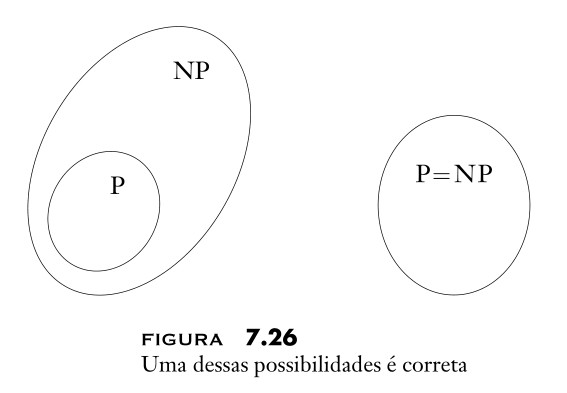
\includegraphics[width=9cm]{images/pNp.png}
		\end{center}
	\end{frame}	
	
	\section{NP-Completude}	
	\begin{frame}{NP-Completude}
		\begin{block}{Teorema de Cook-Levin (7.27)}
			SAT $\in$ {\bf P} se, e somente se, {\bf P} = {\bf NP}.
		\end{block} \pause
		\begin{block}{Teorema 7.31}
			Se A $\leq_P$ B e B $\in$ P, então A $\in$ P.
		\end{block} \pause
		\begin{block}{Teorema 7.32}
			3SAT é redutível em tempo polinomial a CLIQUE.
		\end{block}
	\end{frame}
	
	\begin{frame}{NP-Completude}
		\begin{block}{Definição de NP-Completude}
			Uma linguagem B é NP-completa se ela satisfaz duas condições:
			\begin{enumerate}
				\item B está em NP, e
				\item toda A em NP é redutível em tempo polinomial a B.
			\end{enumerate}
		\end{block} \pause
		\begin{block}{Teorema 7.35}
			Se B for NP-completa e B $\in$ P, então P = NP.
		\end{block} \pause
		\begin{block}{Teorema 7.36}
			Se B for NP-completa e B $\leq_p$ C para C $\in$ NP, então C é NP-completa.
		\end{block}
	\end{frame}
	
	\begin{frame}{P {\it versus} NP}
		\begin{block}{Se P $\subseteq$ NP, então...}
			\begin{center}
				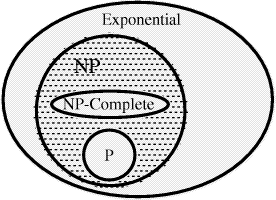
\includegraphics[width=6cm]{images/np_completo2.png}
			\end{center}
		\end{block}		
	\end{frame}	
	
	\begin{frame}
		\titlepage
	\end{frame}
	
\end{document}